\subsection{Comparison of clustering algorithms}
In this section, we will be comparing different clustering algorithms as discussed in the section \ref{clust}. Although only a few results are shown here, they are enough to understand the motive behind choosing the algorithm that performs consistently. The buildings discussed are \texttt{Doug McDonell Building} and \texttt{Redmond Barry Building} for Meeting Room and Toilet Facilities respectively.

\subsubsection {Doug McDonell Building (Parkville Campus) - Meeting Rooms}

As shown in the Appendix Table \ref{appendix:dough.park}, it can be seen that although the budget constraint is the same for KMEANS and MINI KMEANS, the rewards for both the algorithms are different. While the KMEANS result is consistent, whereas the results for MINI KMEANS vary because of the randomness it introduces while selecting the data. Hence the average reward for KMEANS is \texttt{2.07} in both the iterations but it changes from \texttt{1.91} to \texttt{2.07} for MINI KMEANS. Figure \ref{fig:iter1} and \ref{fig:iter2} shows the clustering output by various algorithms across 2 iterations.

\begin{figure}[H]
\centering
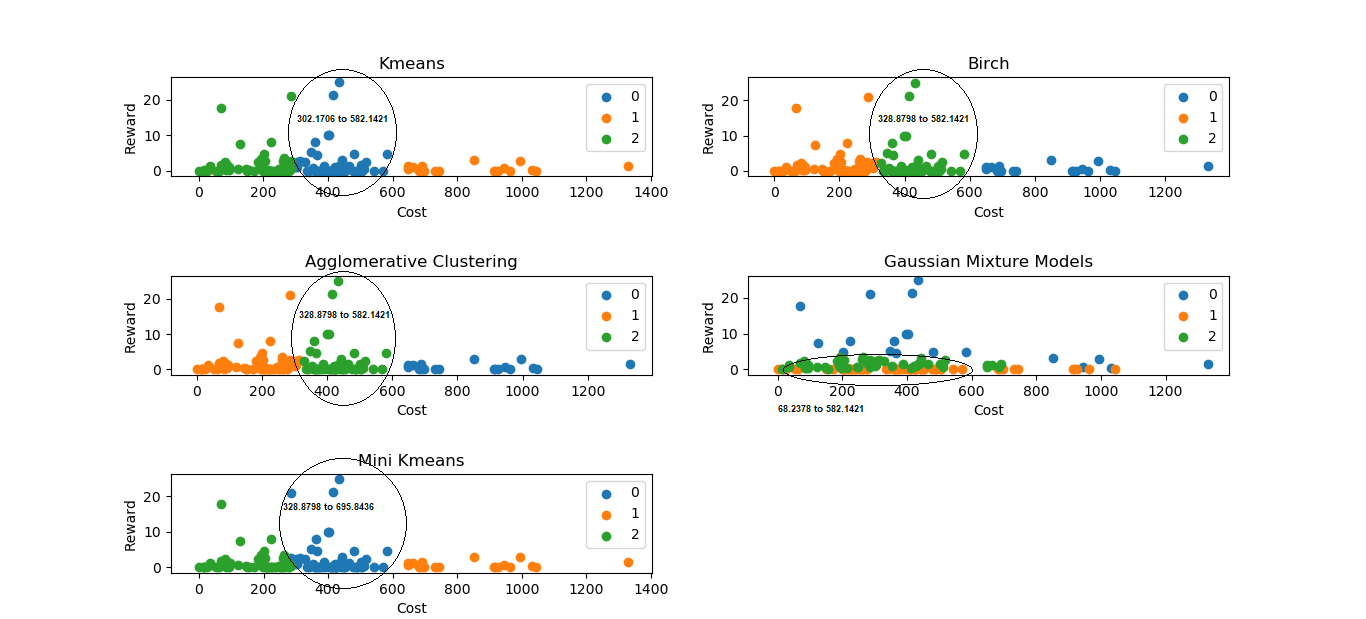
\includegraphics[width=15cm]{resources/168_14.png}
\caption{Comparison of clustering algorithms: Iteration 1}
\label{fig:iter1}
\end{figure}

\begin{figure}[H]
\centering
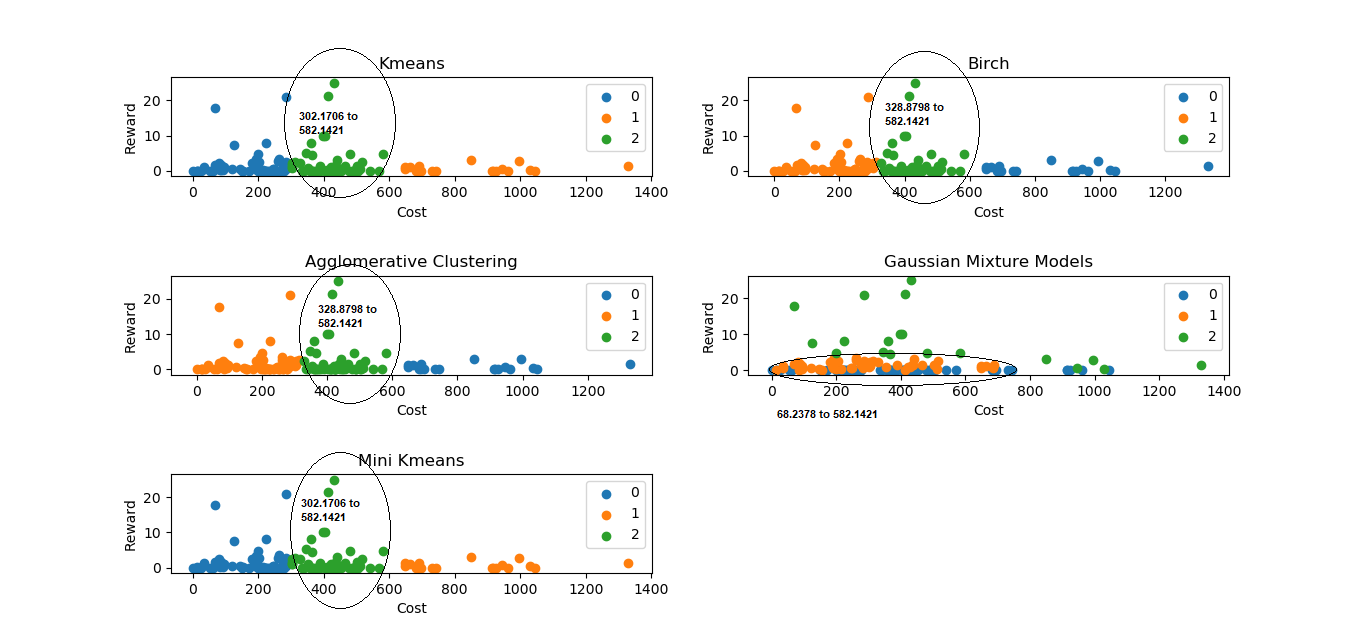
\includegraphics[width=15cm]{resources/168_2.png}
\caption{Comparison of clustering algorithms: Iteration 2}
\label{fig:iter2}
\end{figure}

% \begin{figure}[H]
% \begin{subfigure}{.5\textwidth}
% \centering
%   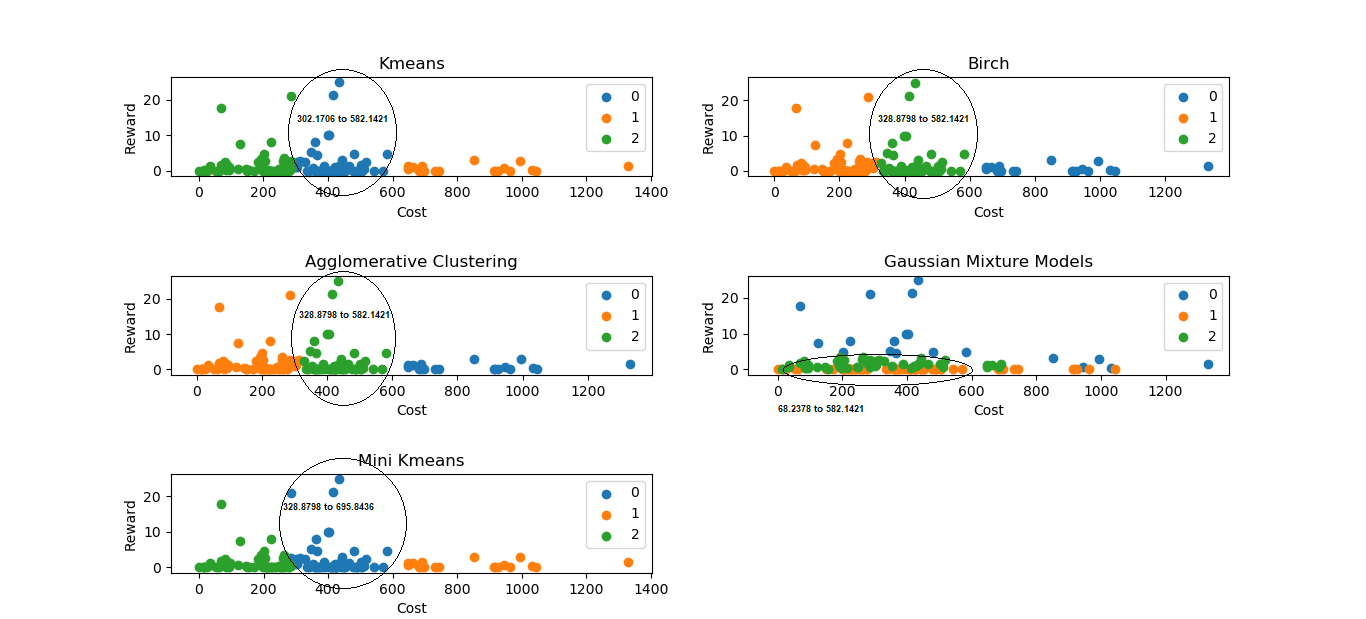
\includegraphics[width=8cm]{resources/168_14.png}
% \end{subfigure}%
% \begin{subfigure}{.5\textwidth}
%   \centering
%   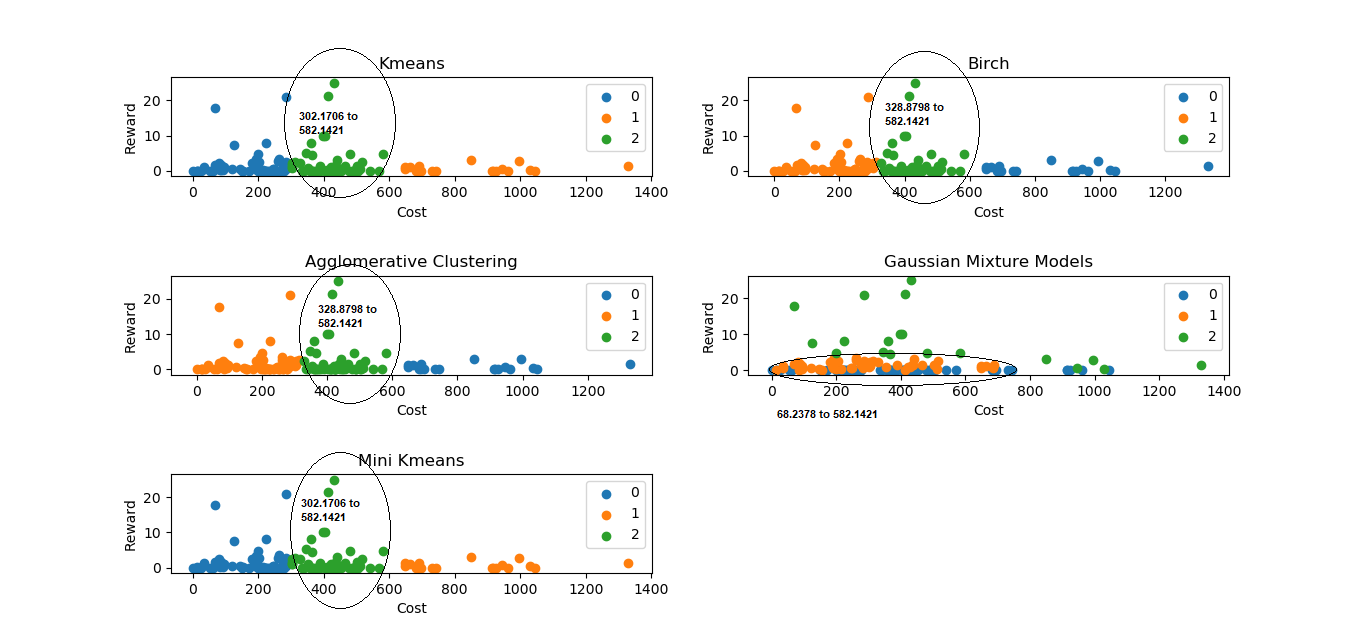
\includegraphics[width=8cm]{resources/168_2.png}
% \end{subfigure}
% \caption{Comparison of clustering algorithms over 2 iterations}
% \label{fig:comp1}
% \end{figure}

\subsubsection {Redmond Barry Building (Parkville Campus) - Toilet Facility}
As shown in the Appendix Table \ref{appendix:red.park}, it can be seen that KMEANS and MINI KMEANS have similar rewards but the budget constraint changes for KMEANS are \texttt{3-422 meters} in both the iteration while for MINI KMEANS it changes from \texttt{3-431} meters to \texttt{3-443} meters.
 Figure \ref{fig:iter3} and \ref{fig:iter4} shows the clustering output by various algorithms across 2 iterations.

\begin{figure}[H]
\centering
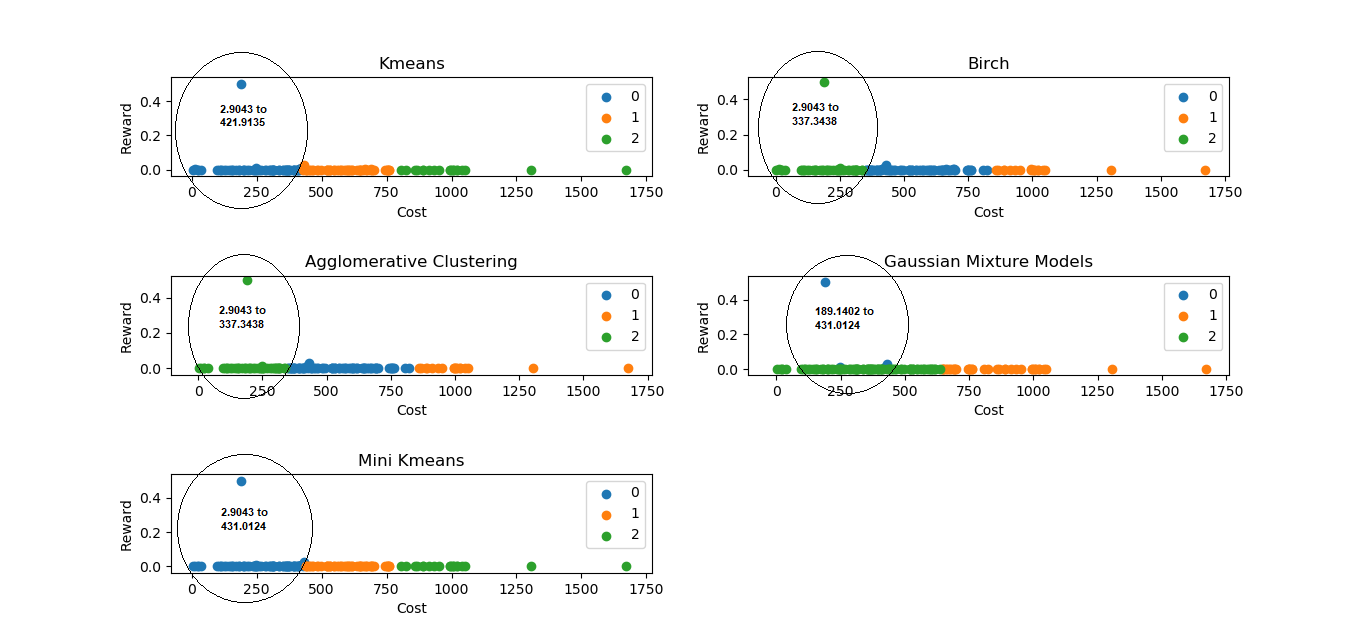
\includegraphics[width=15cm]{resources/115_1.png}
\caption{Comparison of clustering algorithms: Iteration 1}
\label{fig:iter3}
\end{figure}

\begin{figure}[H]
\centering
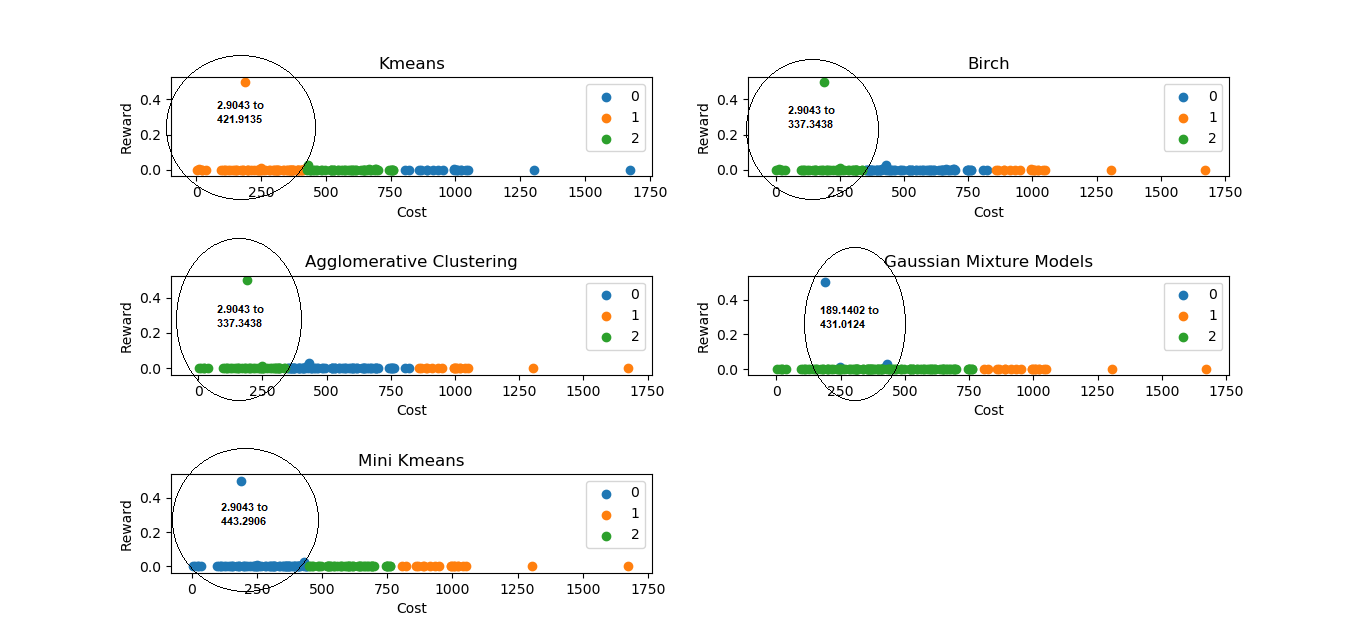
\includegraphics[width=15cm]{resources/115_2.png}
\caption{Comparison of clustering algorithms: Iteration 2}
\label{fig:iter4}
\end{figure}

% \begin{figure}[H]
% \begin{subfigure}{.5\textwidth}
% \centering
%   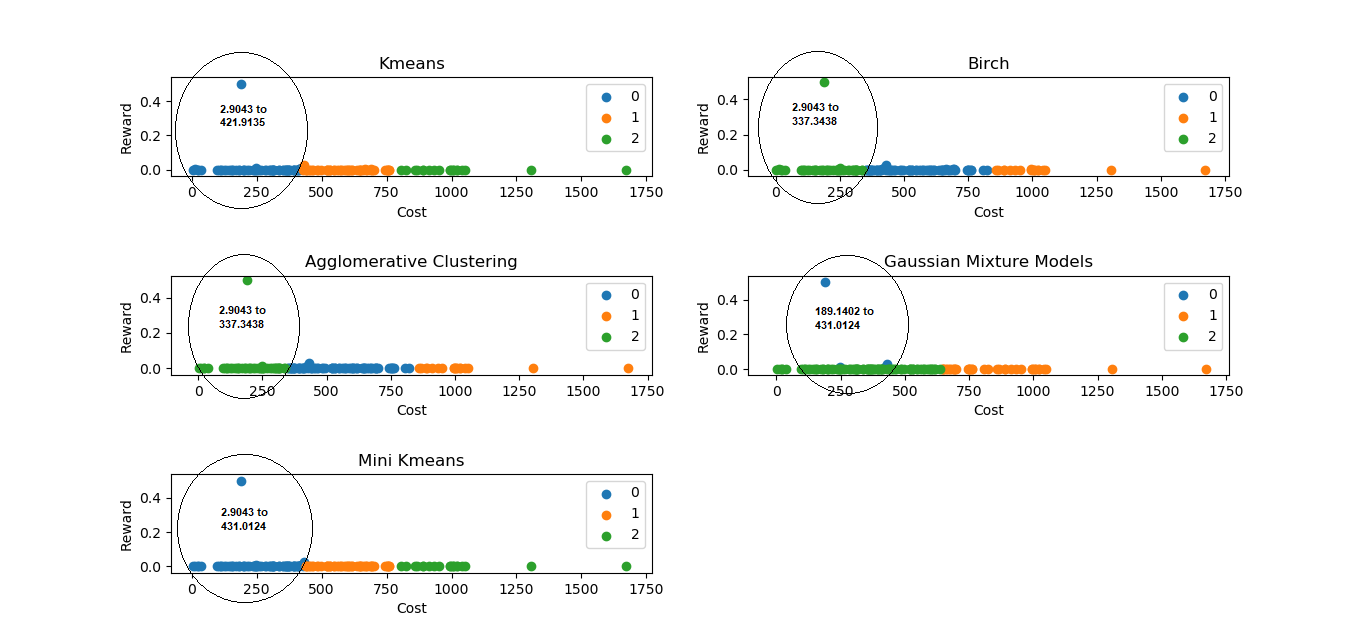
\includegraphics[width=8cm]{resources/115_1.png}
% \end{subfigure}%
% \begin{subfigure}{.5\textwidth}
%   \centering
%   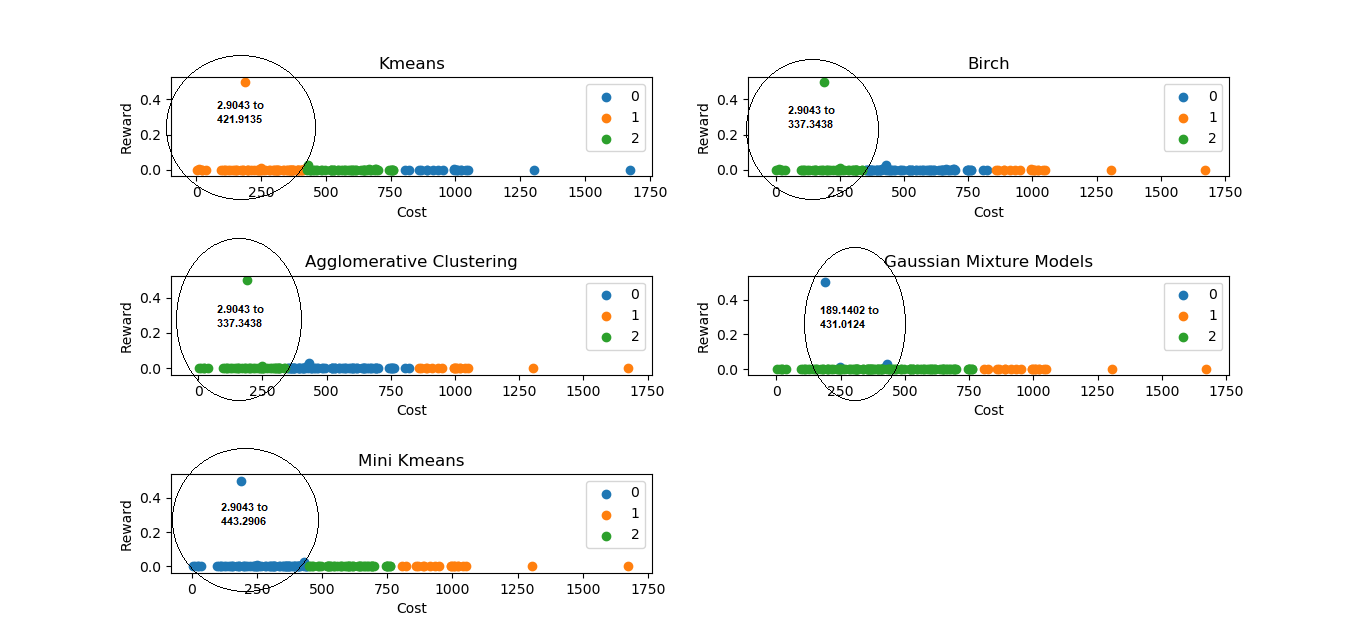
\includegraphics[width=8cm]{resources/115_2.png}
% \end{subfigure}
% \caption{Comparison of clustering algorithms over 2 iterations}
% \label{fig:comp2}
% \end{figure}
